\documentclass{article}
\usepackage[final]{neurips_2018}

\usepackage[utf8]{inputenc} % allow utf-8 input
\usepackage[T1]{fontenc}    % use 8-bit T1 fonts
\usepackage{hyperref}       % hyperlinks
\usepackage{url}            % simple URL typesetting
\usepackage{booktabs}       % professional-quality tables
\usepackage{amsfonts}       % blackboard math symbols
\usepackage{nicefrac}       % compact symbols for 1/2, etc.
\usepackage{microtype}      % microtypography
\usepackage{graphicx}
\usepackage{multicol}
\usepackage{biblatex}
\usepackage{algorithmic}
\usepackage[ruled,vlined]{algorithm2e}
\addbibresource{references.bib}


\setlength{\arrayrulewidth}{0.5mm}
\setlength{\tabcolsep}{18pt}
\renewcommand{\arraystretch}{1.5}

\title{Generative models for Paraphrase Generation}

\author{
  Beomjun Aaron Bae \\
  \texttt{beomjuna@uci.edu} \\
   \And
   Dheeru Dua \\
  \texttt{ddua@uci.edu} \\
   \AND
  Ananth Gottumukkala \\
  \texttt{agottumu@uci.edu} \\
}


\begin{document}

\maketitle

\begin{abstract}

 We are interested in studying deep generative models for paraphrase generation. Most conditional generation models often assign different likelihood to semantically similar(paraphrased) sentences due to left-to-right decoding. We wish to compare the latent representations and performance of Variational Autoencoder (VAE), Generative Adversarial network (GAN) and hybrid VAE-GAN model when trained of sentence paraphrases. The major challenges would involve synchronizing learning rates, steps and module scheduling for different components to achieve a stable learning paradigm. We hope that optimizing the reconstruction on paraphrases would produce latent space where semantically similar sentences (paraphrases) are closer.
  
\end{abstract}

\section{Introduction}
Discriminatively trained language models~\cite{radford2019language} do not have access to future context as a result of which semantically similar sentences often have varied sentence-level log-likelihoods. Non auto-regressive~\cite{ma2019flowseq} models try to solve this problem by predicting token at each position in the sentence but they tend to produce non-grammatical sentence and are very brittle to length of a sentence.

We want to test our hypothesis that a deep generative model trained with a pair of paraphrases can force the latent space mapping of semantically similar sentences close to each other. We compare the performance of three deep generative models: Variational Autoencoder, Generative Adversarial network and a hybrid version of GAN and VAE. The model training setup involves encoding and mapping a sentence to a gaussian latent space, $z$ and decode a paraphrase from it.

We found that GANs so far perform the best for this task. VAE and VAE-GANs suffer from severe mode collapse in the beginning positions(first and second) of sentence positions but surprisingly generate semantically meaningful tokens towards the later part of the sentence.



\section{Data Exploration}
To train and test our models, we decided to use two different datasets. The first is ParaNMT and the second is MS Coco dataset. This section will show how the two datasets are unique and different from one another.
\subsection{ParaNMT} 
ParaNMT is a dataset created by a Wieting et al \cite{wieting2017paranmt50m}. The goal was to create a set of English paraphrase pairs that could be used to find more information about sentence embeddings. They were able to create this dataset by taking Czech sentences from CzEng dataset \cite{Bojar2016CzEng1E} and translating the Czech reference sentence into an English sentence. The ParaNMT dataset includes the original CzEng's English reference sentence and the translated sentence as the two paraphrase sentences. The translation was done via the NMT system of Sennrich et al \cite{sennrich2017nematus}.
The dataset is noted by its relatively short sentences and its ability to have high Pearson correlation coefficients when using some well known embedding models like trigrams and LSTMs. Table 1 shows  some example paraphrase sentences.
\begin{table}
\small
\begin{center}
\begin{tabular}{ |p{2cm}|p{4.5cm}|p{4.5cm}|  }
\hline
\multicolumn{3}{|c|}{Dataset Examples} \\
\hline
Source & Original & Paraphrase \\
\hline
ParaNMT & She's supposed to mark the tents of the pregnant women with white rocks. & to mark the tents of pregnant women with white stones\\
\hline
ParaNMT & the only thing experience teaches us is that experience teaches us nothing & experience teaches us one thing, and though the experience won't teach us anything \\
\hline
MS Coco & A man talking on a phone standing behind a blue car. & An older man sitting on a small pole by a small car with the back open.\\
\hline
MS Coco & a group of three baskets sitting under a stop sign. & Three shopping carts sitting in a parking lot. \\
% \hline
% MS Coco & A cat sits on a chair with eyes closed & A cat that is laying down on a chair.\\
\hline
\end{tabular}
\end{center}
\caption{Samples from ParaNMT and MS Coco}
\end{table}
\par From these examples, you can see that not only are the vocabulary variegated, the sentence structures are also diverse. This is because the parses of the original CzEng sentences were taken into account during the filtering process of the ParaNMT creation. This diverse vocabulary will allow our paraphrase generation models to express in a wider set of sentence embedding space. 
\subsection{MSCOCO}
Microsoft COCO dataset was originally intended for object recognition task in an image \cite{lin2014microsoft}. Thus, the dataset includes iamges of natural scenes that contain specific objects, and these objects are in large categories like "person", "dogs", and etc. However, papers like Gupta et al \cite{gupta2017deep} and Prakash et al \cite{prakash-etal-2016-neural} started to use the captions of the images as paraphrases. This dataset is unique in that it is a dataset of paraphrasese that describe a specific scene and the sentence structure is simplistic. 

As you can see in table 1, MS Coco paraphrases are mostly a noun phrases that describe a specific object in action. However, the words that describe them are variegated like a "cart" versus a "basket". This dataset should be able to provide the needed diversity in vocabulary choices and take advantage of the synonyms that can be found in the annotations.

\section{Model Exploration}
To generate paraphrases, we implemented three different models. Simple VAE based model, a GAN based model, and a third model in combination of both of the models. The architecture and the results are shown in the following sections.


\begin{table*}[t]
    \small
    \centering
    \begin{tabular}{p{0.8cm}p{5.5cm}p{5.5cm}}
        \toprule
            Model & Original Sentence & Perturbed Sentence \\
        \midrule
            VAE &  a lunch counter that serves pizza and drinks. & a living room with a couch , coffee table , television , television and television .\\
            & some women on skiis standing between some trees. & a man and a woman are standing in a kitchen with a dog looking at the camera.\\
          
        \midrule
            GAN & A rural landscape with a farmhouse and grazing cows. & a cow standing in red picture and picture is by head \\
            & Two laptop computers sitting on top of a white desk. & a laptop screens laptop monitors with a speakers\\
            
        \midrule
            VAE- & some players in action on a baseball field & people in action on the baseball field \\
            GAN & a batter about to take a swing at a base ball game & a man is about to hit a swing at a pitch \\
            & a living room with a large rug and couche & a room with a couch and television\\
        \bottomrule
    \end{tabular}
    \label{tab:qual}
    \caption{Sampled Perturbed Sentences from VAE, GAN, and VAE-GAN models}
\end{table*}


\subsection{VAE}
The model that was implemented for a VAE model was largely based on two different papers. The first was Bowman et al \cite{bowman2015generating} and the second was Gupta et al \cite{gupta2017deep}. Although VAE models we studied during class was mostly in the context of image generation, we were able to adopt VAE structure to language generation task, which was largely inspired by Bowman et al. Furthermore, the ability to extend this single sentence learning model can be attributed to Gupta et al. 

The model basically uses two cascading LSTM layers as its encoder and two other LSTM layers as its decoder. The first two LSTM layers encode the original and the paraphrase sentences, respectively, by passing the hidden weights from the original sentence's LSTM as the initial hidden weights of the paraphrase sentence's LSTM. Then, as per usual VAE, the resulting hidden weights are used to create a $\mu$ and a $\sigma$, which are used to create a latent variable $z$. 

Then, on the decoder side, there are two LSTM layers, first of which takes in the original sentence, again, and the second of which takes in the paraphrase sentence. However, the difference here is that the original sentence's LSTM layer use the latent variable $z$ as its initialized hidden input. The loss function is the same as the one shown in Gupta et al's paper, and the inference scheme is simply running the decoder side of the network using a randomly sampled $z$.

However, as great as the initial thoughts were, the performance of this model is not as great as expected. In the table below, poorly generated examples are shown, from both ParaNMT and MS Coco. The results overall lack a strong conditional dependence on the input original sentence. The model trained on ParaNMT largely begins its sentences with the word "I" and the one trained on MS Coco starts with "a man". Although the MS Coco model seems to be able to generate sentences that are within a vicinity, but neither could be considered a proper paraphrases. For example, the last example shows that the model identified the word "standing" to be a key word and it uses it in the generated sentence. However, the overall sentiment is still nowhere close.
\subsection{GAN}
Our GAN model and implementation is based on ~\cite{zhao2018arae}. The ARAE (Adversarially Regularized Autoencoder) GAN trains an autoencoder to generate realistic samples in addition to a generator that creates fake samples. The model first encodes a sentence $x$ into a hidden representation $c$ (using the autoencoder) and then maps it to the $z$ latent space. The input sentence, the target output sentence and a negative target sentence were all encoded this way. In addition to the ARAE GAN implementation, a critic was added and trained alongside the generator, autoencoder and discriminator to predict sentence similarities by minimizing the distance in the $z$ latent space between the source and target sentences while maximizing the distance between the source and negative target sentences. All components of the model were trained with the Wasserstein-GAN objective function.
\subsection{VAE-GAN}
\begin{figure}[htp]
    \centering
    \centering
    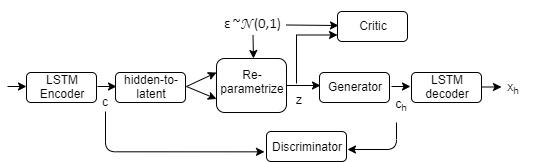
\includegraphics[height=0.25\textwidth,width=\textwidth]{vaegan-Page-1.png}
    \label{fig:vaegan}
    \caption{VAE-GAN hybrid model}
\end{figure}
Our VAE-GAN hybrid model is based on ~\cite{rosca2017variational}. We first, encode a sentence, $x$ into a hidden space representation $c$ and then map it to a gaussian latent space $z$ which is inverted back to $\hat{c}$ via generator network (Figure~\ref{fig:vaegan}). We replace the KL divergence term in ELBO with a critic which tries to estimate the density ratio between the prior density $p(z)$ and generator input density, $q(z|x)$ which is essentially the same thing as KL divergence. The discriminator is a trained in traditional manner by trying to differentiate between real and fake samples. The critic, discriminator and generator are trained with Wasserstein-GAN objective. The algorithm is shown below.

\begin{algorithm}
\begin{algorithmic}
 \item Initialize parameters of generator $\theta$, LSTM Encoder and hidden-to-latent mapping MLP $\eta$, discriminator(D) $\phi$ and critic(C) $\omega$ randomly. Prior distribution $p(z) \sim N(0,1)$ \\
 \WHILE {i< |epochs|}
 \item Update parameters $\eta$ by minimizing loss = CrossEntropy(x, $x_h$) + $(c_h - c)^2$ - $E_x[C(\hat{z})]$, where $\hat{z} \sim q_\eta(z|x)$ \\
 \item Update parameters $\phi$ by minimizing $E_z[D(G(z_p))] + E_x[D(\hat{c})] - E_x[D(c)]]$, where $z_p \sim p(z))$ \\
 \item Update parameters $\omega$ by minimizing $E_x[C(z)] - E_z[C(z_p)]$ \\
 \ENDWHILE
 \caption{Pseudo-code VAE-GAN}
 \end{algorithmic}
\end{algorithm}

We also add gradient penalty to critic and discriminator. We tried a variety of learning rates and learning schedules to balance the interaction of critic, discriminator and generator but couldn't achieve Nash equilibrium. 

\section{Results and Discussion}
We compare various models by computing accuracy of generated paraphrase with the reference target paraphrase. This measure is a very strict as the model can generate correct paraphrases but still not get full score. Table~\ref{tab:quant} and show Table~\ref{tab:qual} show quantitative and qualitative  results on ParaNMT and MS-COCO.

\begin{table}
\centering
\small
\begin{tabular}{ccc}
    \toprule
     Model & MS COCO & ParaNMT  \\
     \midrule
     VAE & 9.3 & 4.2 \\
     GAN & 26.4 & 51.5 \\
     VAE-GAN & 58.6 & 43.3\\
     \bottomrule \\
\end{tabular}
\label{tab:quant}
\caption{Test Accuracy results}
\end{table}

 




\section{Contributions}
\begin{enumerate}
    \item[-] Beomjun Aaron Bae was responsible for creating and testing the VAE portion of the project.
    \item[-] Ananth Gottumukkala was responsible for creating and testing the GAN portion of the project.
    \item[-] Dheeru Dua was responsible for creating and testing the VAE-GAN portion of the project.
\end{enumerate}

\printbibliography

\end{document}
